\section{Development Technology}

For the client-side hardware, we used a Raspberry Pi with the PN532 NFC/RFID controller breakout board. This acts as our NFC-enabled device which will be used to read and write to the tags. The tags we used are generic brand NFC tags available on Amazon.ca. We implemented the client-side functionality using Python and the NFCpy library to read and write information from NFC tags. It also allowed us to be able to cleanly parse and manipulate the data within our code. The Raspberry Pi is running the Raspberrian OS that is designed to be used on the Pi. After reading through documentation on the PN532 NFC/RFID board we were able to connect to the board using UART and the Raspberry Pi’s serial port. Once this was achieved, the NFCpy library was able to connect to the device using the serial port’s tty path.

\begin{figure}[H]
    \centering
    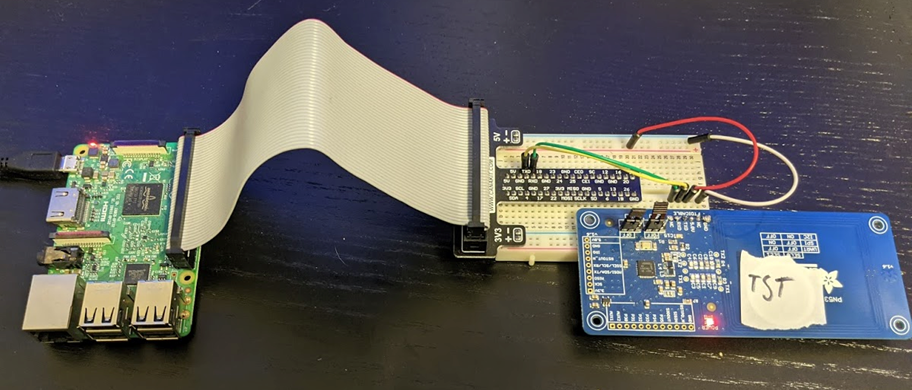
\includegraphics[width=\textwidth]{figures/hardware_setup.png}
    \caption{Client-side hardware setup}
\end{figure}

The NodeJS server is also running on the Raspberry Pi. The NodeJS server will act as the main authentication system that will receive data from the NFC-enabled client. The API functions replicate the algorithm that is outlined within the paper. Our API is able to check the hash values sent from the device to compare the values stored in the database then the API verifies the device, generates a random value to write to the tag, generates a response hash for the device, and generates a hash that contains the new tag value. Most of the computing power is done on the server-side as the hashes are computed and compared to be valid on the server.

\begin{figure}[H]
    \centering
    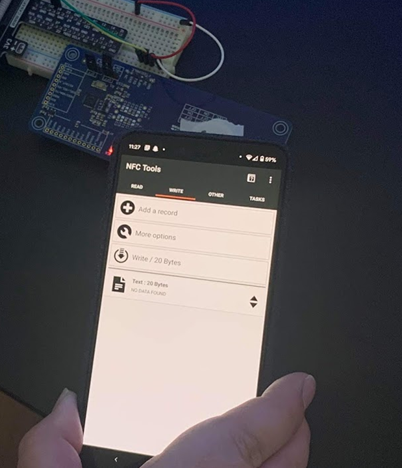
\includegraphics[width=3in]{figures/nfctools.png}
    \caption{NFCTools editing tag information}
\end{figure}

For the database, all necessary information needed to be stored to authenticate these components use the SQLite3 database on the same Raspberry Pi as the server. We used a NodeJS module called sqlite3 which allows us to interact with the SQLite3 database on the server. This module allows us to be able to read, write, delete, and update entries within the database. The database is read and written to from the NodeJS server that sends information to the client device for authentication. 
